% Source: graduate-coursework/Prior_Semesters/Fa25/EMCH501/HW1/HW1.tex

\documentclass[border=4pt]{standalone}
\usepackage{amsmath}
\usepackage{amssymb}
\usepackage{graphicx}
\usepackage{tikz}
\usepackage{xcolor}
\usetikzlibrary{shapes.geometric, arrows.meta, positioning, decorations.pathmorphing, patterns}

\begin{document}
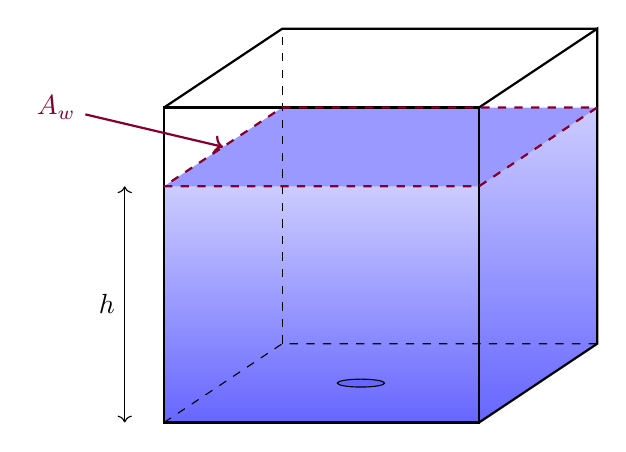
\begin{tikzpicture}
        % Coordinates
        \coordinate (A) at (0,0);
        \coordinate (B) at (4,0);
        \coordinate (C) at (4,4);
        \coordinate (D) at (0,4);
        \coordinate (E) at (1.5,1);
        \coordinate (F) at (5.5,1);
        \coordinate (G) at (5.5,5);
        \coordinate (H) at (1.5,5);

        % Water level
        \coordinate (W1) at (0,3);
        \coordinate (W2) at (4,3);
        \coordinate (W3) at (5.5,4);
        \coordinate (W4) at (1.5,4);

        % Shading for water
        \fill[blue!40, bottom color=blue!60, top color=blue!20] (A) -- (B) -- (W2) -- (W1) -- cycle;
        \fill[blue!40, bottom color=blue!60, top color=blue!20] (B) -- (F) -- (W3) -- (W2) -- cycle;
        \fill[blue!40] (W1) -- (W2) -- (W3) -- (W4) -- cycle;


        % Back hidden lines
        \draw[dashed] (A) -- (E) -- (F);
        \draw[dashed] (E) -- (H);

        % Visible lines
        \draw[thick] (A) -- (B) -- (C) -- (D) -- cycle;
        \draw[thick] (B) -- (F) -- (G) -- (C);
        \draw[thick] (D) -- (H) -- (G);

        % Hole
        \draw[fill=blue!60] (2.5, 0.5) ellipse (0.3 and 0.05);

        % Water surface outline
        \draw[dashed, thick, purple!70!black] (W1) -- (W2) -- (W3) -- (W4) -- cycle;

        % Labels
        \draw[<->] (-0.5,0) -- (-0.5,3);
        \node[left] at (-0.5,1.5) {$h$};
        \node[left, text=purple!70!black] at (-1, 4) (Aw_label) {$A_w$};
        \draw[->, thick, purple!70!black] (Aw_label) -- (0.75, 3.5);

    \end{tikzpicture}
\end{document}
